\section{Struktura danych \textsc{KMS(s)}}
\label{sec:kms}
Pokażemy strukturę $KMS(s)$ z pracy \cite{kriz05}, parametryzowaną po $s$, która dla statycznej tablicy $A[1:n]$ będzie wspierała poniższe operacje:
\begin{enumerate}[nosep]
    \item \textsc{count}$(x,i,j)$ -- zwraca $F^A_x(i,j)$ w czasie $\Oh(\log n)$
    \item \textsc{query}$(i,j)$ -- zwraca dominantę i jej częstotliwość na przedziale $A[i:j]$ w czasie $\Oh(n/s \log n)$
\end{enumerate}
\subsection{Konstrukcja struktury \textsc{KMS(s)}}
\begin{figure}[H]
    \centering
    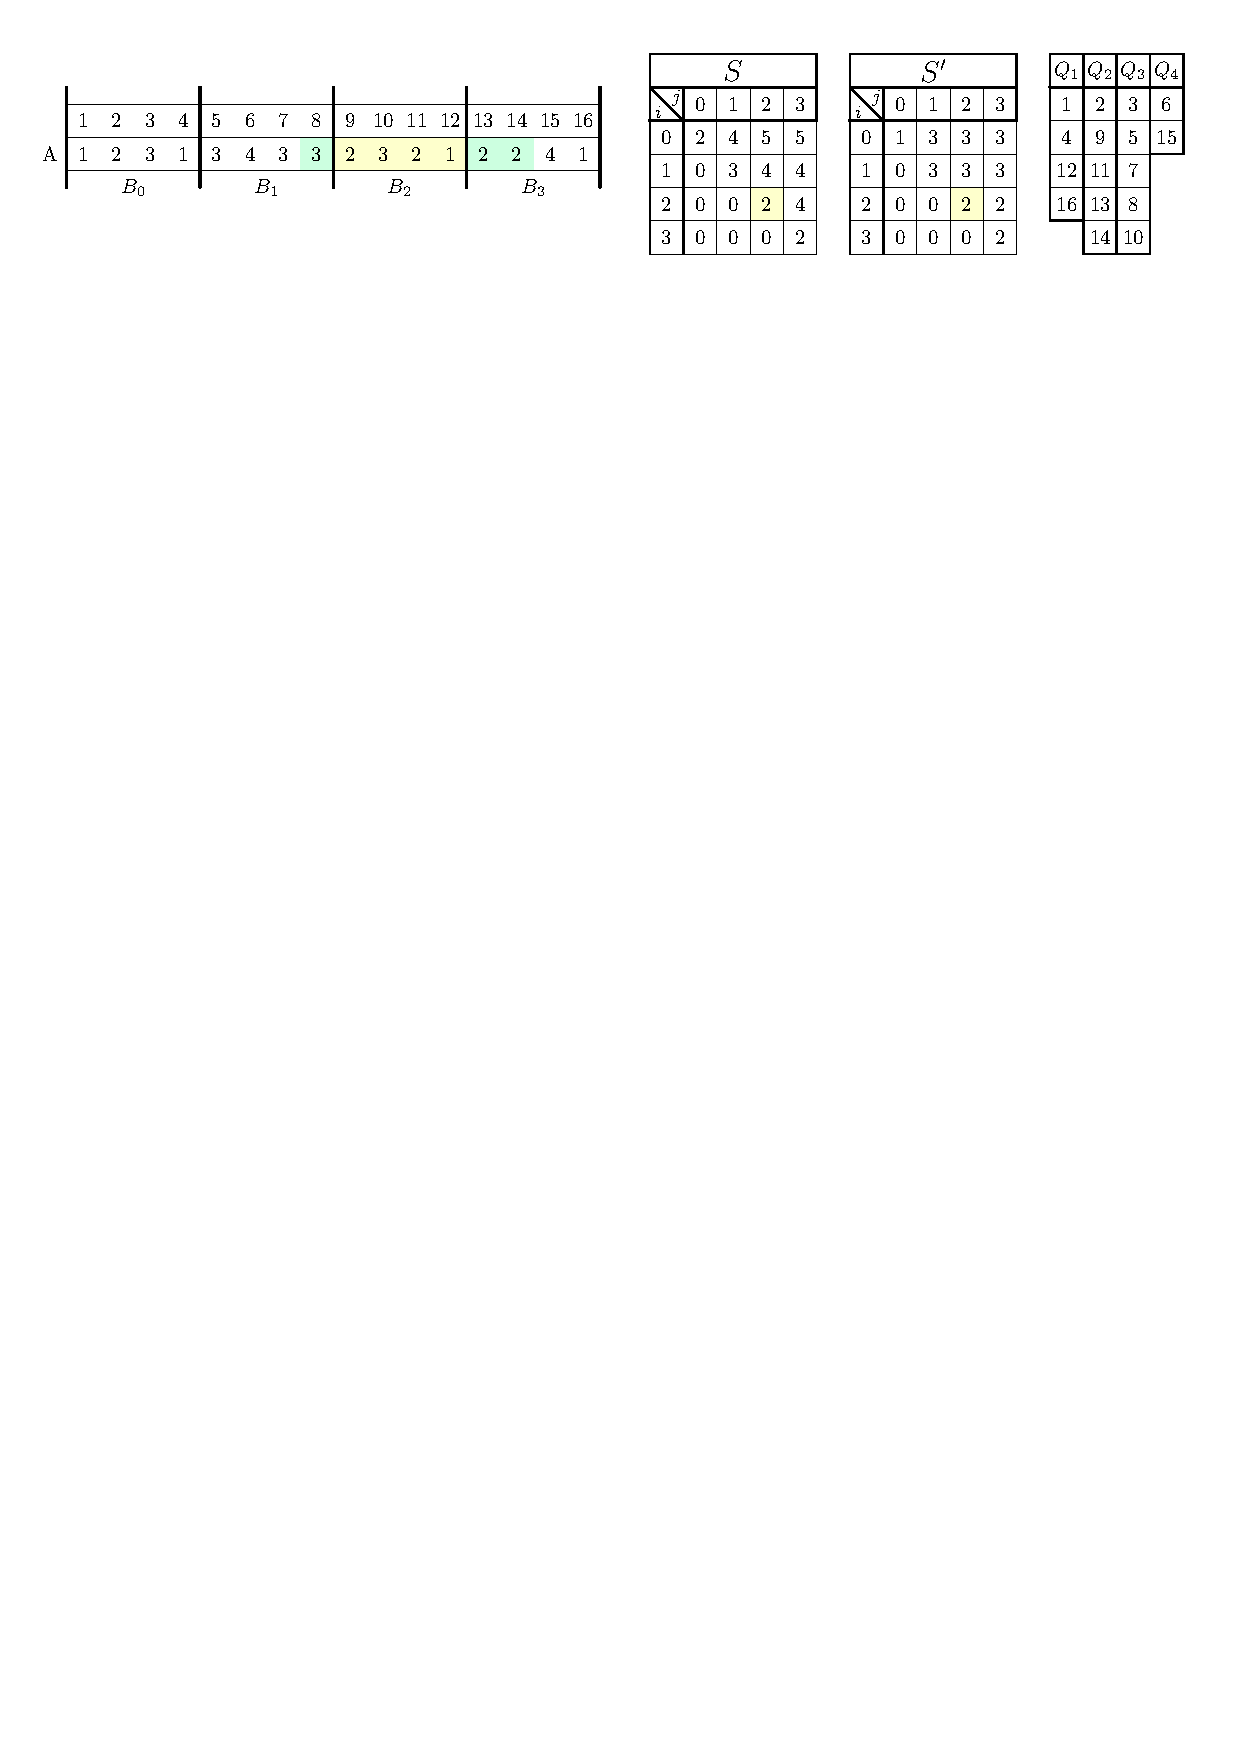
\includegraphics[scale=0.85]{images/kms.pdf}
    \caption{Przykładowa tablica $A[1:16]$ z liczbą unikalnych elementów $\dt=4$ i podziałem na $s=4$ bloki, każdy o rozmiarze $t=4$. Ponadto zaznaczamy zapytanie o dominantę $A[8:14]$ z rozbiciem na prefiks $A[8:8]$, środek $A[9:12]$ oraz sufiks $A[13:14]$, które są zaznaczone odpowiednio kolorami zielonym, żółtym i zielonym.}
    \label{fig:kms}
\end{figure}
Tworzymy $\dt$ tablic $Q_x[0:F^A_x(1,n)-1]$ dla każdego unikalnego elementu $x \in \{1,2,\dots,\dt\}$. Tablica $Q_x$ na $i$-tej pozycji przechowuje indeks $(i+1)$-tego wystąpienia wartości $x$ w tablicy $A$, innymi słowy $Q_x[i] = j \Longleftrightarrow A[j] = x \land F^A_x(1,j) = i+1$. Ponadto dzielimy tablicę $A$ na $s$ bloków, każdy, prócz ostatniego, o rozmiarze $t=\cl{n/s}$. $i$-ty blok $B_i$ dla $i=0,1,\dots,s-1$ reprezentuje przedział $A[it+1, \min(n,(i+1)t)]$. Dla każdej pary bloków $B_i$, $B_j$ przechowujemy w tablicy dwuwymiarowej $S[i,j]$ dominantę multizbioru $B_{i,j} = B_i \cup B_{i+1} \cup \dots \cup B_{j}$. Ponadto przechowujemy tablicę dwuwymiarową $S'[i,j]$, która odpowiada częstotliwości dominanty $S[i,j]$ w multizbiorze $B_{i,j}$.
\subsection{Operacja \textsc{count}}
\begin{algorithm}
    \caption{Operacja \textsc{count}}
    \label{alg:kms-count}
    \begin{algorithmic}[1]
        \Function{count}{$x$,$i$,$j$}
            \State $m \gets$ binary\_search$(Q_x, i)$
            \State $l \gets$ binary\_search$(Q_x, j+1)$
            \State \Return{$l-m$}
        \EndFunction
    \end{algorithmic}
\end{algorithm}
Najpierw pokażemy jak można dla dowolnej wartości $x \in \{1, 2, \dots, \dt\}$ obliczyć jej częstotliwość na przedziale $A[i:j]$ w czasie $\Oh(\log n)$. Oznaczmy przez $x_0 < x_1 < \dots < x_{k-1}$ indeksy wszystkich wystąpień wartości $x$ w przedziale $A[i:j]$. Ponieważ tablica $Q_x$ jest rosnąca, wystąpienia $x_0,\dots,x_{k-1}$ odpowiadają spójnemu fragmentowi tablicy $Q_x[l:l+k-1]$, gdzie $Q_x[l+o] = x_o$ dla $o\in\{0,1,\dots,k-1\}$. Możemy łatwo znaleźć $l$ używając wyszukiwania binarnego, jest to pierwsza wartość w tablicy $Q_x$ większa bądź równa od $i$. Analogicznie szukamy indeksu $m$ następnika $x_{k-1}$ w tablicy $Q_x$, jest to pierwsza wartość większa niż $j$. W przypadku kiedy $k=0$ przyjmujemy $l=m=1$, oraz w przypadku kiedy $x_{k-1}$ jest ostatnim wystąpieniem wartości $x$ w tablicy $A$ przyjmujemy $m=F^A_x(1,n)$. Teraz łatwo zauważyć, że $F^A_x(i,j) = m-l$. Dla przykładu rozważmy wartość 2 na przedziale $A[8:14]$ w rysunku \ref{fig:kms}. dwa występuje 4 razy na tym przedziale, na indeksach $x_0=9,x_1=11,x_2=13,x_3=14$, które odpowiadają przedziałowi $Q_2[1:4]$. Używając binarnego wyszukiwania możemy szybko znaleźć indeksy $l=1$ oraz $m=5$ odpowiadające $x_0$ oraz następnikowi $x_3$ w tablicy $Q_2$. Z indeksów $m, l$ można obliczyć częstotliwość elementu $2$ na przedziale $A[8:14]$: $F^A_2(8,14)=l-m=5-1=4$.

\subsection{Operacja \textsc{query}}
\begin{algorithm}[t]
    \caption{Operacja \textsc{query}}
    \label{alg:kms-query}
    \begin{algorithmic}[1]
        \Function{query}{$i$,$j$}
            \State mfreq $\gets 0$
            \State mmode $\gets 0$
            \If{$j-i \le t$}
                \For{k $\gets i,i+1,\dots j$}
                    \State freq $\gets$ count$(A[k], i, j)$
                    \If{freq $>$ mfreq}
                        \State mfreq $\gets$ freq
                        \State mmode $\gets A[k]$
                    \EndIf
                \EndFor
                \State \Return mfreq, mmode
            \EndIf
            \State $b_i \gets \fl{(i-1)/t}$
            \State $b_j \gets \fl{(j-1)/t}$
            \If{$b_i+1 \le b_j-1$}
                \State mfreq $\gets$ S'[$b_i+1,b_j-1$]
                \State mmode $\gets$ S[$b_i+1,b_j-1$]
            \EndIf
            \For{k $\in$ prefiks $\cup$ sufiks}
                    \State freq $\gets$ count$(A[k], i, j)$
                    \If{freq > mfreq}
                        \State mfreq $\gets$ freq
                        \State mmode $\gets A[k]$
                    \EndIf
                \EndFor
            \State \Return freq, mode
        \EndFunction
    \end{algorithmic}
\end{algorithm}
\begin{lemma}
\label{lem:1}
(\cite{kriz05}) Niech $A, B, C$ będą multizbiorami. Jeżeli dominanta $A \cup B \cup C$ nie jest w $A$, ani w $C$ to jest nią dominanta multizbioru $B$.
\end{lemma} 

\hspace{-1em}Zapytanie o dominantę na przedziale $A[i:j]$ podzielimy na 2 przypadki w zależności od rozmiaru przedziału.
W pierwszym przypadku gdy $j-i \le t$, iterujemy się liniowo po elementach przedziału
$A[i:j]$ (linijki 4-10) i liczymy ich częstotliwość używając operacji \textsc{count}. Zwracamy element o maksymalnej częstotliwości. \\
W drugim przypadku, gdy $j-i > t$, elementy $A[i]$ oraz $A[j]$ znajdują się w różnych blokach. Oznaczmy przez $b_i=\fl{(i-1)/t}, b_j=\fl{(j-1)/t}$ odpowiednio numery bloków do jakich należą elementy $A[i]$ oraz $A[j]$. Dzielimy $A[i:j]$ na trzy części $A[i:(b_i+1)t]$, $A[(b_i+1)t+1:b_jt]$ oraz $A[b_jt+1:j]$. Nazwijmy pierwszą i ostatnią część prefiksem i sufiksem. Wtedy z lematu \ref{lem:1} wiemy, że dominantą $A[i:j]$ jest dominanta środkowej części lub któryś z elementów prefiksu lub sufiksu. Dominantę środkowej części przechowujemy w $S[b_i+1,b_j-1]$ (linijki 11-15). Prefiks i sufiks mają ograniczony rozmiar przez $t$, więc obsługujemy te dwa fragmenty tak jak w przypadku pierwszym (linijki 16-21). 
\subsection{Analiza złożoności czasowej}
\paragraph{Konstrukcja} Tablice $Q_i$ można stworzyć podczas jednego skanowania tablicy $A$ co kosztuje $\Oh(n)$ czasu. $i$-te wiersze tablic $S[i,*], S'[i,*]$ możemy stworzyć liniowo skanując tablicę $A$. Wierszy w tablicach S oraz S' jest s. Łącznie na konstrukcje tablic S, S' potrzebujemy $O(sn)$ czasu. W takim razie, konstrukcja struktury \textsc{KMS(s)} zajmuje $\Oh(n + sn) = \Oh(sn)$ czasu.
\paragraph{Operacja \textsc{count}} Jak wspomniano wcześniej, operacja \textsc{count} trwa $\Oh(\log n)$ czasu, ponieważ używa dwóch binarnych wyszukań na danych o wielkości $\Oh(n)$.
\paragraph{Operacja \textsc{query}} W pierwszym przypadku, gdy $j-i \le t$ operacja \textsc{query} wykonuje $\Oh(t)$ operacji \textsc{count}, każda trwa po $\Oh(\log n)$ czasu, zatem przypadek pierwszy zabiera co najwyżej $\Oh(t \log n)$ czasu. W drugim przypadku wykonujemy operacje \textsc{count} iterując się po prefiksie i sufiksie. Prefiks jak i sufiks mają ograniczony rozmiar przez $\Oh(t)$. Łącznie drugi przypadek trwa $\Oh(t \log n)$ czasu. Oba przypadki łącznie zajmują $\Oh(t \log n + t \log n) = \Oh(t \log n)$ czasu.
\subsection{Analiza złożoności pamięciowej}
\paragraph{Konstrukcja} Podczas konstrukcji tworzymy $\dt$ tablic $Q_i$, które łącznie zajmują $\Oh(n)$ pamięci. Ponadto tworzymy dwie dwuwymiarowe tablice S oraz S' każda o rozmiarze $\Oh(s^2)$. Łącznie struktura danych zajmuje $\Oh(n + s^2)$ pamięci.\paragraph{Operacje \textsc{count} i \textsc{query}} Obie wspierane operacje używają stałej pamięci.

\subsection{Dobór parametru s}
Podstawiając $s=n^{1-e}$ dla $e \in (0, 1/2]$ Otrzymujemy strukturę danych o czasie konstrukcji $\Oh(n^{2-e})$, która zajmuje $\Oh(n^{2-2e})$ pamięci. Pozwala ona na obliczenie dominanty w czasie $\Oh(n^e \log n)$. W szczególności dobierając $e=1/2$ dostajemy liniową pamięć i $\Oh(\sqrt{n} \log n)$ czas zapytania.

\newpage